\chapter{Результаты экспериментальных исследований безвинтового подводного робота с внутренними роторами}\label{ch:ch4}

\section{Методика проведения экспериментальных исследований}\label{sec:ch4/sec1}

Эксперименты проводились в бассейне размерами 3 х 1.5 x 1.5 метра, заполненным водой. При движении робота траектория отслеживалась с помощью системы захвата движения фирмы Contemplas, которая состоит из 4 камер, расположенных по периметру области съемки. Камеры предназначены для работы под водой. 

Для работы с системой камер используется программное обеспечение Vicon Motus и Templo. Перед каждой серией экспериментов система калибруется, используя специальный калибровочный объект, который состоит из штатива, центрального куба и штанг с маркерами. Система калибруется, используя известные из документации координаты маркеров. Фото бассейна с установленными камерами и калибровочным объектом в центре представлено на рисунке~\ref{Pool}.

\begin{figure}[h]
	\centering
	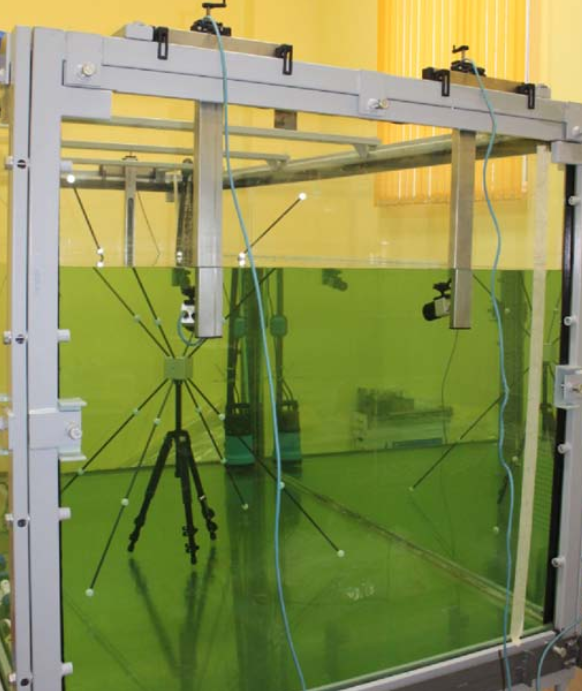
\includegraphics[width=0.5\linewidth]{Pool.png}%
	\caption{Фото бассейна с установленными камерами и калибровочным объектом}
	\label{Pool}
\end{figure}

При проведении экспериментальных исследований на отслеживаемый объект устанавливаются маркеры таким образом, чтобы в каждый момент времени каждый маркер был в кадре минимум двух камер. После записи и обработки видео получаем траекторию движения объекта и проекции единичных векторов, связанных с осями подвижной системы координат, расположенной на объекте на глобальную неподвижную систему координат. Данные проекции образуют матрицу поворота объекта, которая связывает неподвижную и подвижную системы координат. Съемка ведется с частотой 50 Гц.

\section{Проведение экспериментальных исследований}\label{subsec:ch4/sec2/sub1}

\subsection{Эксперименты с погружением безвинтового подводного робота с внутренними роторами}
Цель экспериментов -- проверить работоспособность связки "модули плавучести--датчики давления", а также алгоритмы управления данными модулями для погружения и всплытия безвинтового подводного робота.

Рассмотрим эксперимент с погружением робота на 0.4 метра и дальнейшим всплытием. Для погружения оба модуля плавучести параллельно начинают набор воды, пока значение глубины, получаемое с датчиков давления не будет равно заданному. Начальное и конечное положение робота при погружении представлено на рисунке~\ref{BPRUpDown}а. Для всплытия оба модуля плавучести сливают набранную воду и полностью освобождают свои емкости. Начальное и конечное положение робота при всплытии представлено на рисунке~\ref{BPRUpDown}б.

\begin{figure}[!ht]
	\begin{minipage}[h]{0.5\linewidth}
		\center{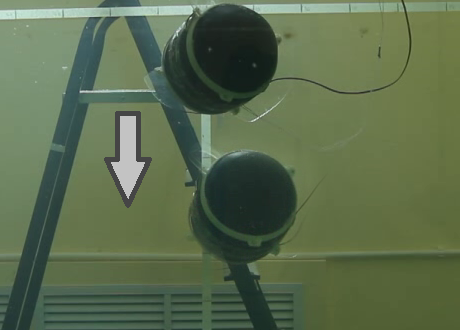
\includegraphics[height=0.7\linewidth]{BPRGoDown.png} }
	\end{minipage}
	\hfill
	\begin{minipage}[h]{0.5\linewidth}
		\center{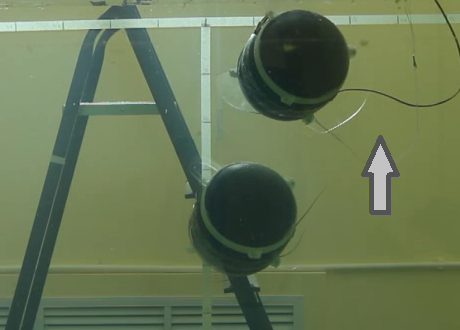
\includegraphics[height=0.7\linewidth]{BPRGoUp.png} }
	\end{minipage}
	
	\begin{minipage}[h]{0.5\linewidth}
		\center{а}
	\end{minipage}
	\hfill
	\begin{minipage}[h]{0.5\linewidth}
		\center{б}
	\end{minipage}
	
	\caption{Начальное и конечное положение робота при погружении (а) и всплытии (б)}
	\label{BPRUpDown}
\end{figure}

Видеозапись описанного эксперимента можно посмотреть по следующей ссылке: https://youtu.be/\_daOZjUeq2Q

\subsection{Эксперименты с движением безвинтового подводного робота с внутренними роторами}

Цель экспериментов -- определение характера движения безвинтового подводного робота при различных управляющих воздействиях. В качестве управляющих воздействий выступают гиростатические моменты роторов K1, K2, K3, возникающие при их вращении. Рассмотрены три серии экспериментов: вращение только пары больших роторов, вращение только одной пары меньших роторов и одновременное вращение пары больших и одной пары меньших роторов. В каждом эксперименте роторы разгонялись до максимальной скорости 590 об/мин.

Так как роторы 2 и 3 имеют одинаковые массо-геометрические характеристики и лежат в одной плоскости, их совместное вращение приведет к качественно аналогичному, результату, что и в случае их вращения по отдельности.


\textbf{Вращение пары больших роторов.} В качестве управляющего воздействия выступала угловая скорость пары больших роторов, ось вращения которых совпадает с большей полуосью эллипсоида. Роторы разгонялись до максимальной скорости 590 об/мин, которая поддерживалась постоянной в течение 3 секунд. Вектор внутреннего гиростатического момента, сообщенный телу после разгона роторов, $K = (2i_1\omega_{max}, 0, 0)$. Положение робота в начальный момент времени и момент времени $t=3$ секунды после начала движения, для отдельного эксперимента представлено на рисунке \ref{BPR_exp1}.

\begin{figure}[h]
	\begin{minipage}[h]{0.5\linewidth}
		\center{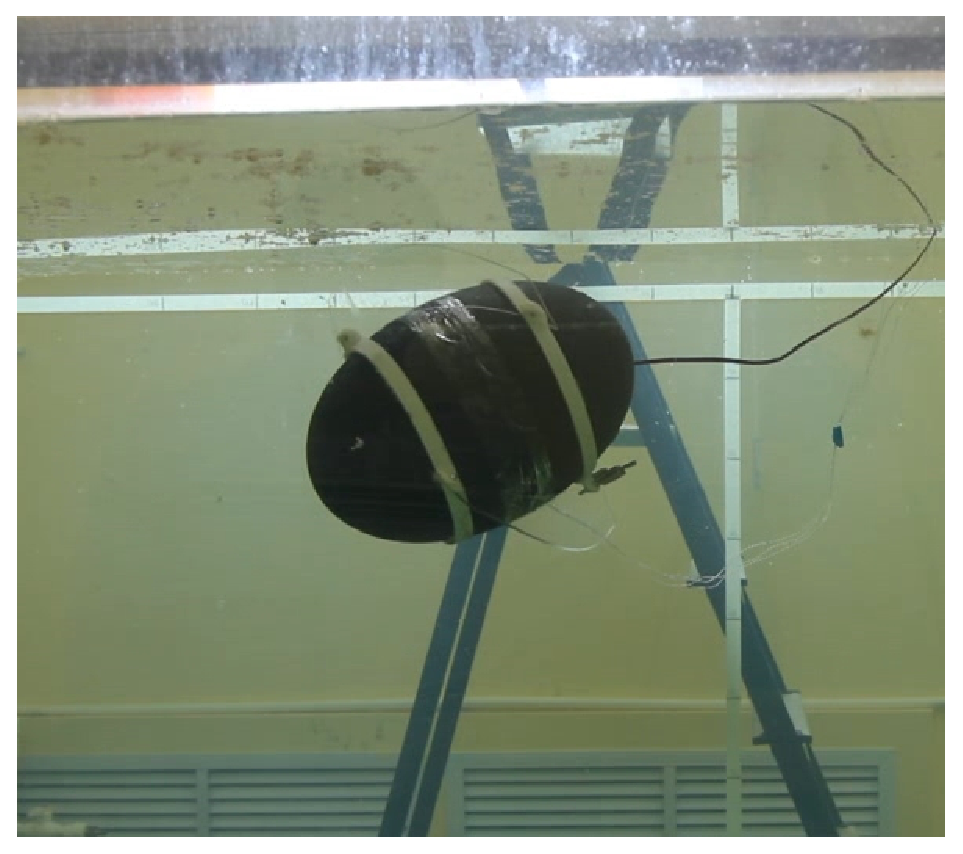
\includegraphics[width=0.7\linewidth]{exp11.eps} \\ а)}
	\end{minipage}
	\begin{minipage}[h]{0.5\linewidth}
		\center{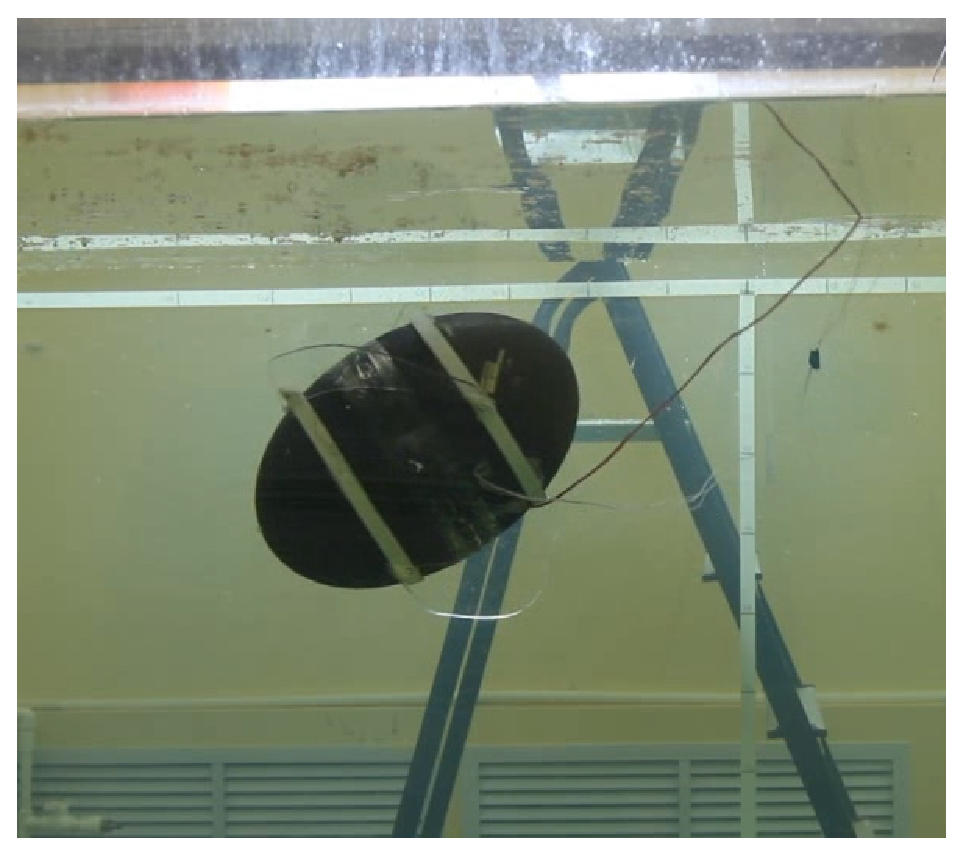
\includegraphics[width=0.7\linewidth]{exp12.eps} \\ б)}
	\end{minipage}
	\caption{Положение робота а) в начальный момент времени и б) момент времени t=3 секунды от начала движения при $\bK=(2i_1\omega_{max},  0,  0)$ }
	\label{BPR_exp1}
\end{figure}

Для данных управляющих воздействий проведена серия из трех экспериментов. Среднее изменение координат геометрического центра робота и изменение углов, определяющих положение, для трех экспериментов составили:

\begin{center}
$\Delta x_{exp}=0.115 \;\mbox{м},\; \Delta y_{exp}=0.010\; \mbox{м},\; \Delta z_{exp}=0.055\; \mbox{м};$ \\ 
$\Delta \theta_{exp}=4^{\circ},\; \Delta \psi_{exp}=10^{\circ},\; \Delta \varphi_{exp}=120^{\circ}.$
\end{center}

Здесь и далее $x_{exp},\;y_{exp},\;z_{exp}$ --- координаты геометрического центра безвинтового подводного робота, $\theta_{exp}$ --- угол дифферента --- угол между осью вращения эллипсоида и горизонтальной плоскостью; $\psi_{exp}$ --- угол курса --- угол между осью вращения эллипсоида и вертикальной плоскостью (этот угол сходен с углом курса судна, но отсчитывается в соответствии с выбранной системой координат); $\varphi_{exp}$ --- угол вращения --- угол, определяющий поворот робота вокруг оси вращения эллипсоида.

Видеозапись описанного эксперимента можно посмотреть по следующей ссылке: https://youtu.be/QzusvCTFpGw

%Траектории движения полученные в результате численного моделирования при вышеописанных управляющих воздействиях и экспериментальные траектории движения робота представлены на рисунке \ref{Exp_BPR_1}.
%
%\begin{figure}[ht]
%	\centering
%	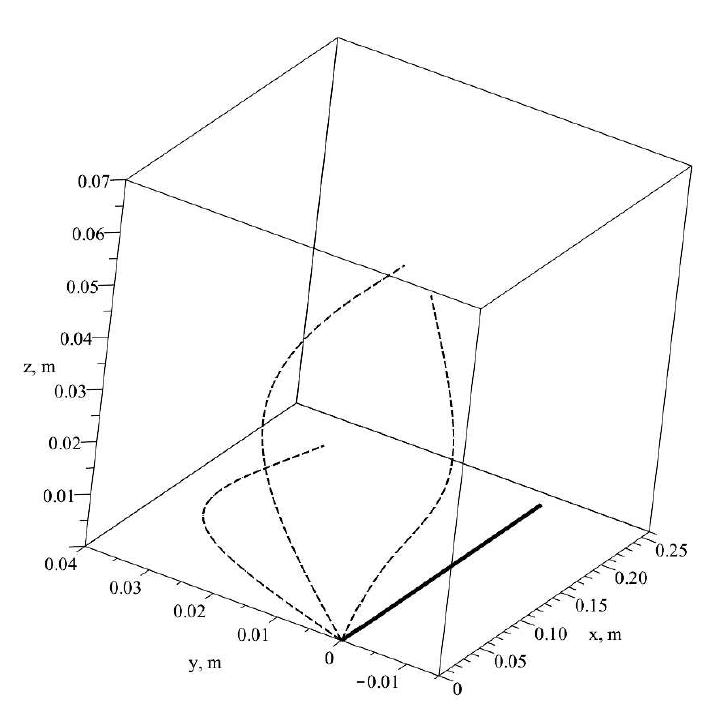
\includegraphics[width=0.5\linewidth]{Exp_BPR_1.png}%
%	\caption{Теоретическая (сплошная линия) и экспериментальные (штриховые линии) траектории движения безвинтового подводного робота при $K = (2i_1\omega_{max}, 0, 0)$}
%	\label{Exp_BPR_1}
%\end{figure}


\textbf{Вращение одной пары малых роторов.} В качестве управляющего воздействия выступала угловая скорость одной пары малых роторов. Роторы разгонялись до максимальной скорости 590 об/мин, которая поддерживалась постоянной в течение 3 секунд. Вектор гиростатического момента, сообщенный телу после разгона роторов, $K = (0, 2i_2\omega_{max}, 0)$. Положение робота в начальный момент времени и момент времени $t=3$ секунды после начала движения, для отдельного эксперимента представлено на рисунке \ref{BPR_exp2}.

% Разгон маховика до данной скорости выполняется за время $t_{acc}=0.7$ с.

\begin{figure}[h]
	\begin{minipage}[h]{0.5\linewidth}
		\center{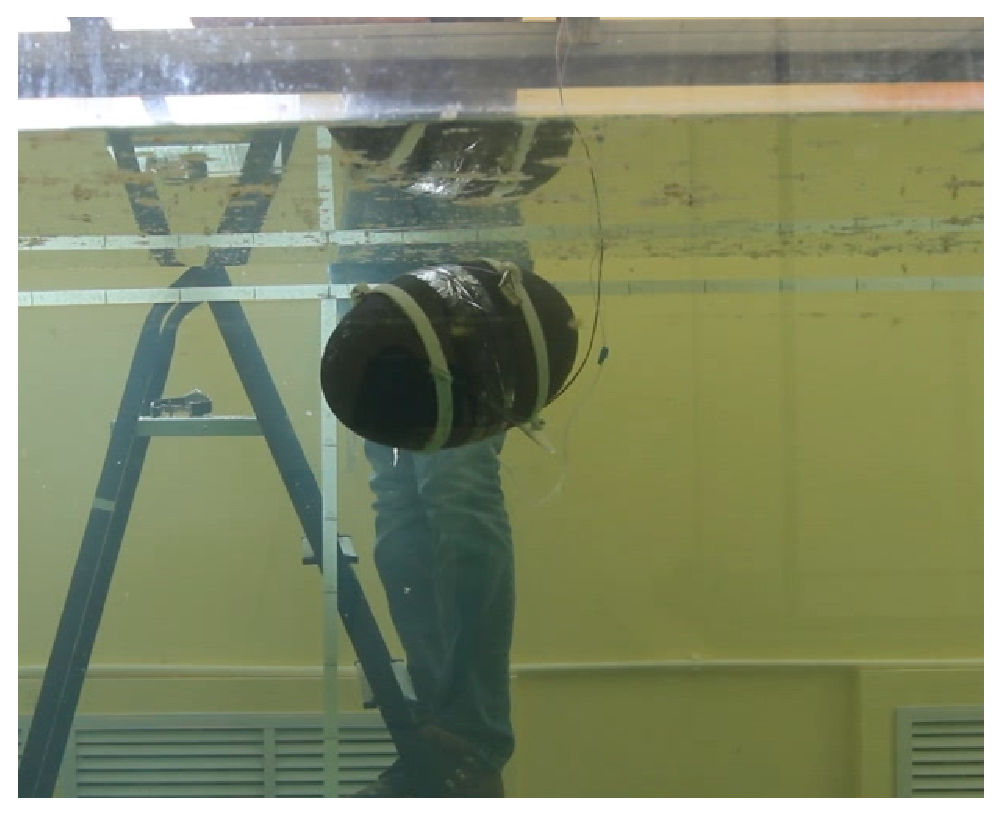
\includegraphics[width=0.7\linewidth]{exp21.eps} \\ а)}
	\end{minipage}
	\begin{minipage}[h]{0.5\linewidth}
		\center{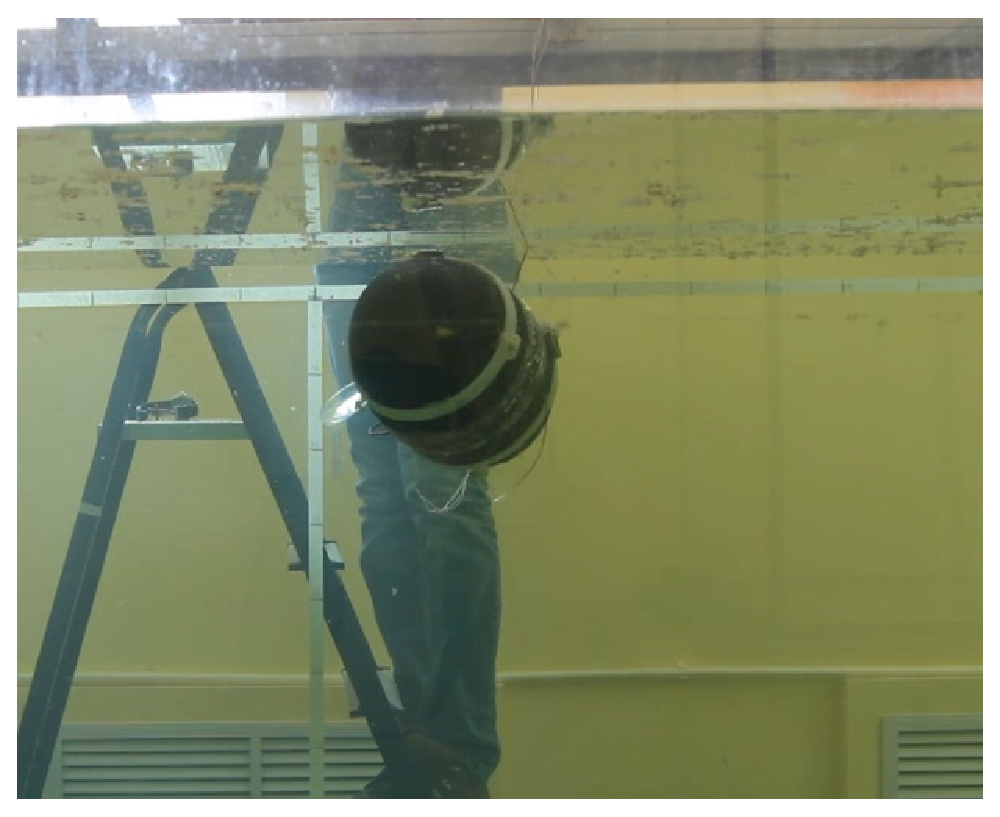
\includegraphics[width=0.7\linewidth]{exp22.eps} \\ б)}
	\end{minipage}
	\caption{Положение робота а) в начальный момент времени и б) момент времени t=3 секунды от начала движения при $\bK=(0,  2i_2\omega_{max}, 0)$}
	\label{BPR_exp2}
\end{figure}

Для данных управляющих воздействий проведена серия из трех экспериментов. Среднее изменение координат геометрического центра робота и изменение углов, определяющих положение, для данной серии экспериментов составили:

\begin{center}
$\Delta x_{exp}=0.054\; \mbox{м},\; \Delta y_{exp}=0.008\,\; \mbox{м},\; \Delta z_{exp}=0.068\; \mbox{м},\;$ \\
$\Delta \theta_{exp}=61^{\circ},\; \Delta \psi_{exp}=62^{\circ},\; \Delta \varphi_{exp}=10^{\circ}.$
\end{center}

Видеозапись описанного эксперимента можно посмотреть по следующей ссылке: https://youtu.be/WSAkAkAhqxQ
%Траектории движения полученные в результате численного моделирования при вышеописанных управляющих воздействиях и экспериментальные траектории движения робота представлены на рисунке \ref{Exp_BPR_2}.
%
%\begin{figure}[ht]
%	\centering
%	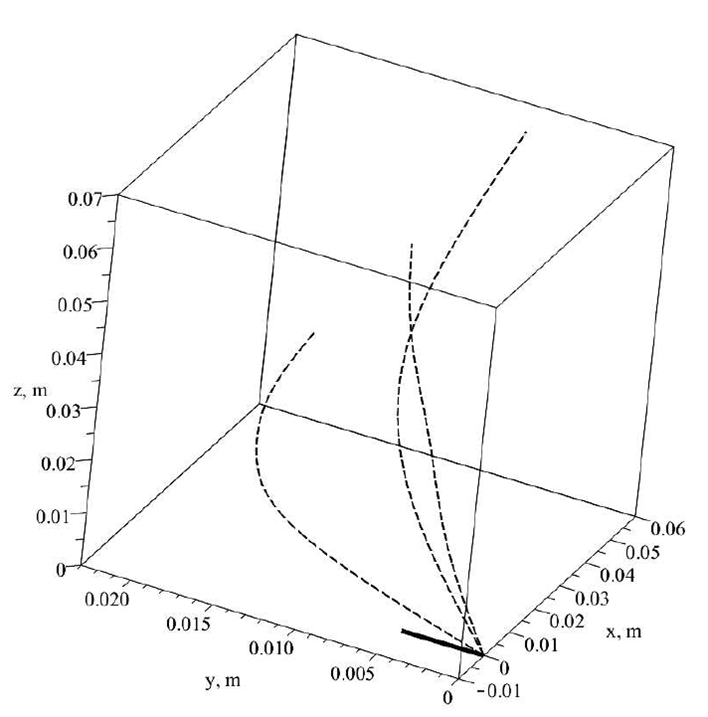
\includegraphics[width=0.5\linewidth]{Exp_BPR_2.png}%
%	\caption{Теоретическая (сплошная линия) и экспериментальные (штриховые линии) траектории движения безвинтового подводного робота при $K = (0, 2i_2\omega_{max}, 0)$}
%	\label{Exp_BPR_2}
%\end{figure}


3.	Вращение пары больших роторов и одной пары малых роторов. В качестве управляющего воздействия выступала угловая скорость одной пары малых и пары больших роторов. Роторы разгонялись до максимальной скорости 590 об/мин, которая поддерживалась постоянной в течение 3 секунд. Вектор гиростатического момента, сообщенный телу после разгона роторов, $K = (2i_1\omega_{max}, 2i_2\omega_{max}, 0)$. Положение робота в начальный момент времени и момент времени $t=3$ секунды после начала движения, для отдельного эксперимента представлено на рисунке \ref{BPR_exp3}.

\begin{figure}[h]
	\begin{minipage}[h]{0.5\linewidth}
		\center{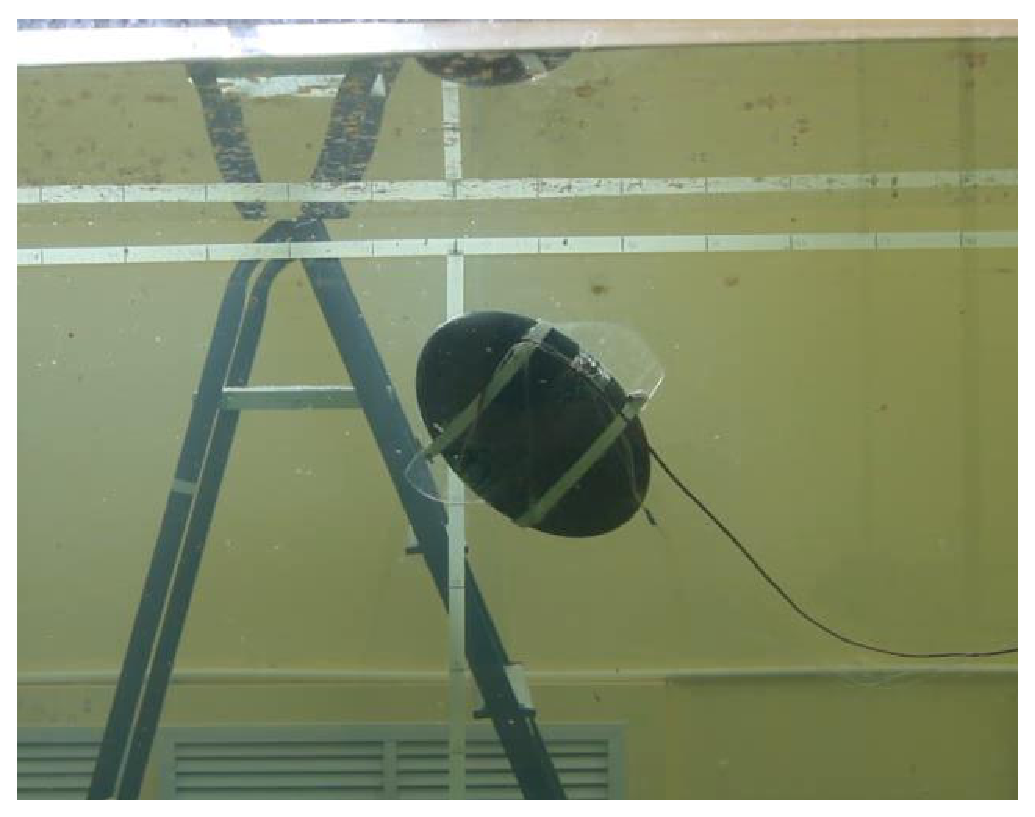
\includegraphics[width=0.7\linewidth]{exp31.eps} \\ а)}
	\end{minipage}
	\begin{minipage}[h]{0.5\linewidth}
		\center{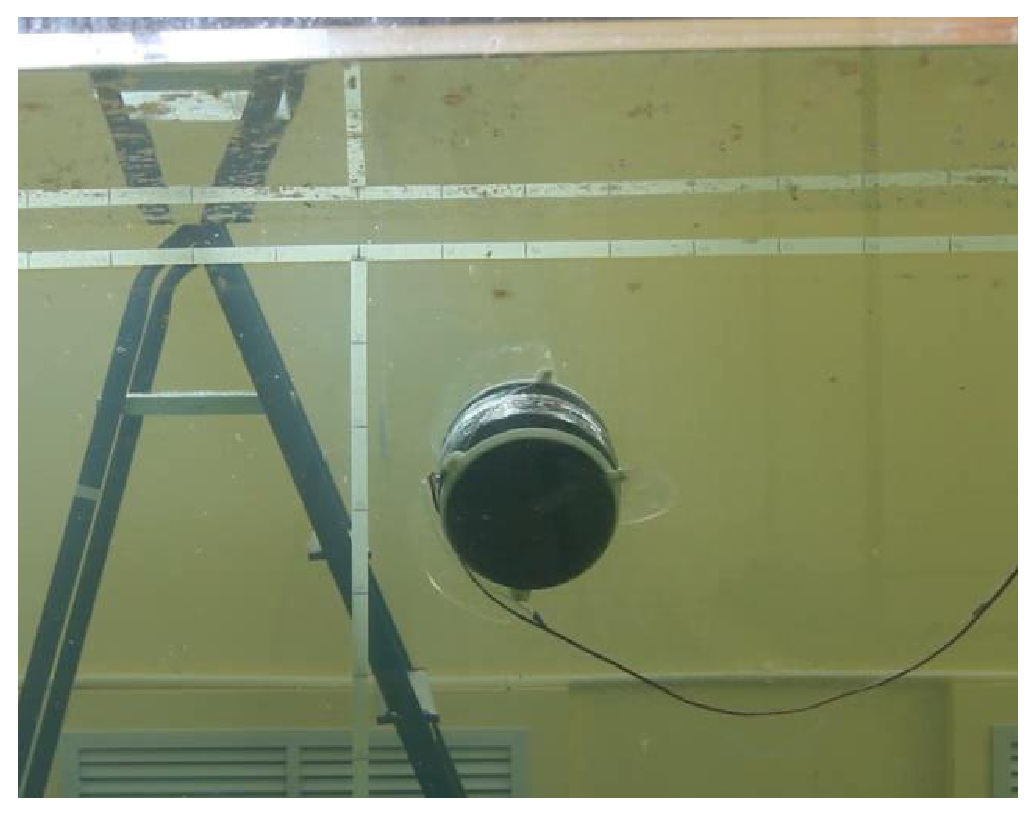
\includegraphics[width=0.7\linewidth]{exp32.eps} \\ б)}
	\end{minipage}
	\caption{Положение робота а) в начальный момент времени и б) момент времени t=3 секунды от начала движения при $\bK=(2i_1\omega_{max}, 2i_2\omega_{max}, 0)$}
	\label{BPR_exp3}
\end{figure}

Для данных управляющих воздействий проведена серия из трех экспериментов. Среднее изменение координат геометрического центра робота и изменение углов, определяющих положение, для данной серии экспериментов составили:

\begin{center}
$\Delta x_{exp}=0.106\; \mbox{м}, \; \Delta y_{exp}=0.050\; \mbox{м},\; \Delta z_{exp}=0.053\; \mbox{м}, \;$ \\
%\item $|r|=0.129$ м;
$\Delta \theta_{exp}=17^{\circ},\; \Delta \psi_{exp}=90^{\circ},\; \Delta \varphi_{exp}=51^{\circ}.$
\end{center}

Видеозапись описанного эксперимента можно посмотреть по следующей ссылке: https://youtu.be/z1go7sthVMc

%Траектории движения полученные в результате численного моделирования при вышеописанных управляющих воздействиях и экспериментальные траектории движения робота представлены на рисунке \ref{Exp_BPR_3}.
%
%\begin{figure}[ht]
%	\centering
%	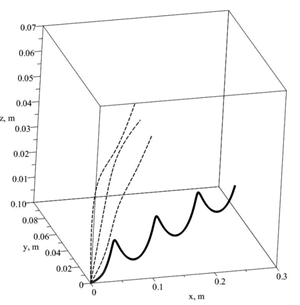
\includegraphics[width=0.5\linewidth]{Exp_BPR_3.png}%
%	\caption{Теоретическая (сплошная линия) и экспериментальные (штриховые линии) траектории движения безвинтового подводного робота при $K = (2i_1\omega_{max}, 2i_2\omega_{max}, 0)$}
%	\label{Exp_BPR_3}
%\end{figure}

Проведенные эксперименты подтвердили возможность реализации движения в жидкости за счет изменения внутреннего гиростатического момента.

%Несмотря на указанную теоретическую возможность перемещения подводного робота с помощью вращения роторов, экспериментальные данные существенно отличаются от результатов, полученных в рамках модели идеальной жидкости. Например, при первых двух вариантах управляющих воздействий в рамках теоретической модели робот движется прямолинейно не изменяя своей ориентации. При проведении экспериментов такого движения добиться не удается. Кроме того, перемещение безвинтового подводного робота на практике в два раза меньше теоретического.

\section{Оценка экспериментальных данных}\label{subsec:ch4/sec2/sub2}

\textbf{1. Вращение пары больших роторов.} Траектория движения, полученная в результате численного моделирования при управляющих воздействиях, заданных в виде $\bK=\begin{pmatrix} 2i_1\omega_{max},  0,  0 \end{pmatrix}$, и экспериментальная траектория движения приведены на рисунке \ref{traj1}. После движения с заданными управляющими воздействиями в течение 3 секунд линейная и угловая скорость составили $\bV_t=\begin{pmatrix} 0.0916,  0, 0 \end{pmatrix}$ м/с, ${\bOm}_t=\begin{pmatrix} 41.0125, 0, 0 \end{pmatrix}$ об/мин. А изменение его ориентации  определяется углами: $\Delta \theta_t=0^{\circ},\; \Delta \psi_t=0^{\circ},\; \Delta \varphi_t=738.2^{\circ}$. При данном управляющем воздействии по результатам численного моделирования, робот проходит расстояние $|\br_t|=0.275$ м, а среднее значение перемещения по экспериментальным данным $|\br_{exp}|=0.128$ м.


\begin{figure}[h!]
	\begin{center}
		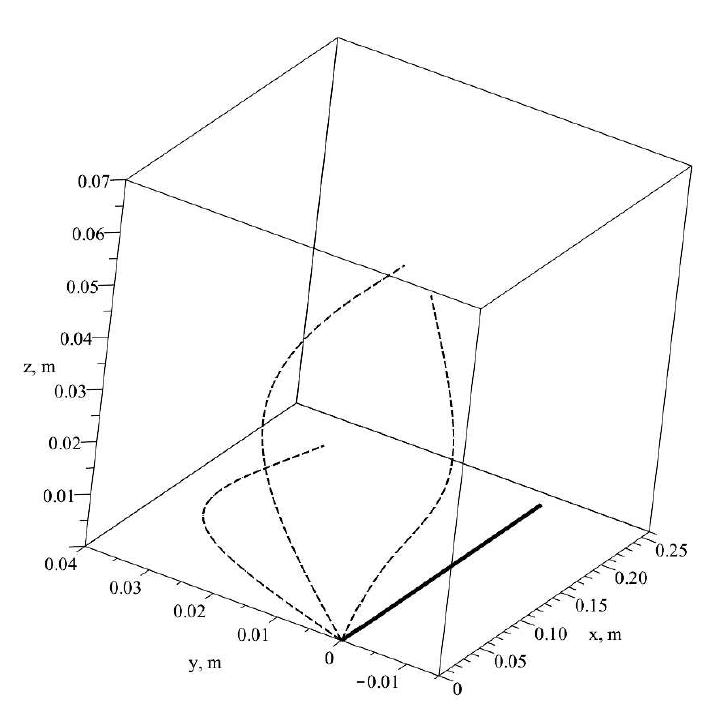
\includegraphics[width=0.5\linewidth]{Exp_BPR_1.png}
		\caption{Теоретическая (сплошная линия) и экспериментальные (штриховые линии) траектории движения безвинтового подводного робота при $\bK=(2i_1\omega_{max},  0,  0)$} 
		\label{traj1}
	\end{center}
\end{figure}

\textbf{2. Вращение одной пары малых роторов.} Траектория движения, полученная в результате численного моделирования при управляющих воздействиях, заданных в виде $\bK=\begin{pmatrix} 0,  2i_2\omega_{max}, 0 \end{pmatrix}$, и экспериментальная траектория движения, приведены на рисунке \ref{traj2}. После движения с заданными управляющими воздействиями в течение 3 секунд линейная и угловая скорость составили $\bV_t=\begin{pmatrix} 0, 0.0018, 0 \end{pmatrix}$ м/с, ${\bOm}_t=\begin{pmatrix} 0, 1.9436, 0 \end{pmatrix}$ об/мин. А изменение его ориентации  определяется углами: $\Delta \theta_t=35^{\circ}, \; \Delta \psi_t=0^{\circ}, \; \Delta \varphi_t=0^{\circ}$. При данном управляющем воздействии по результатам численного моделирования, робот проходит расстояние $|\br_t|=0.005$ м, а среднее значение перемещения по экспериментальным данным $|\br_{exp}|=0.087$ м.

\begin{figure}[h!]
	\begin{center}
		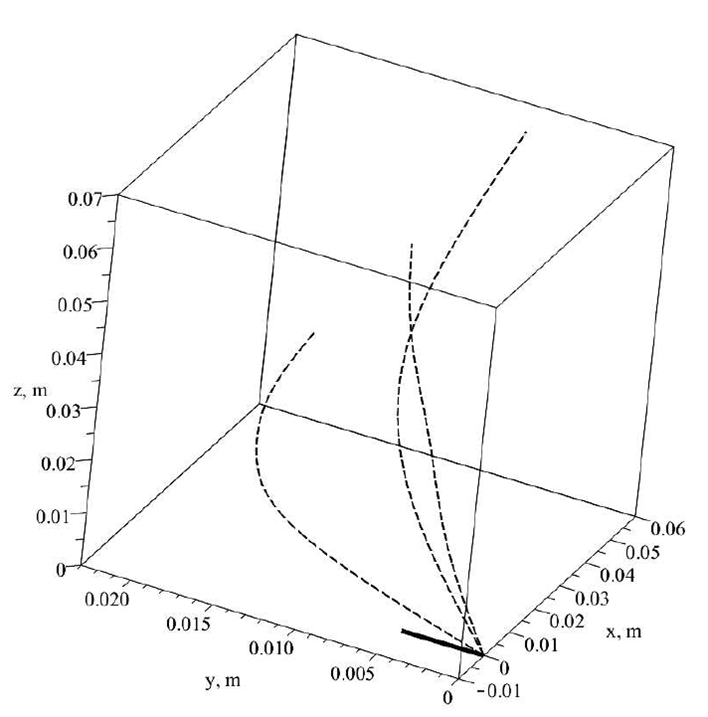
\includegraphics[width=0.5\linewidth]{Exp_BPR_2.png}
		\caption{Теоретическая (сплошная линия) и экспериментальные (штриховые линии) траектории движения безвинтового подводного робота при $\bK=( 0,  2i_2\omega_{max}, 0 )$} \label{traj2}
	\end{center}
\end{figure}

\textbf{3.	Вращение пары больших роторов и одной пары малых роторов.} Траектория движения, полученная в результате численного моделирования при управляющих воздействиях, заданных в виде $\bK=\begin{pmatrix} 2i_1\omega_{max}, 2i_2\omega_{max}, 0 \end{pmatrix}$, и экспериментальная траектория движения, приведены на рисунке \ref{traj3}. После движения с заданными управляющими воздействиями в течение 3 секунд линейная и угловая скорость составили $\bV_t=\begin{pmatrix} 0.0916,  0.0018, 0 \end{pmatrix}$ м/с, ${\bOm}_t=\begin{pmatrix} 41.0125, 1.9436, 0 \end{pmatrix}$ об/мин. А изменение его ориентации  определяется углами: $\Delta \theta_t=35^{\circ}, \; \Delta \psi_t=0^{\circ}, \; \Delta \varphi_t=738.2^{\circ}$. При данном управляющем воздействии по результатам численного моделирования, робот проходит расстояние $|\br_t|=0.275$ м, а среднее значение перемещения по экспериментальным данным $|\br_{exp}|=0.129$ м.

\begin{figure}[h!]
	\begin{center}
		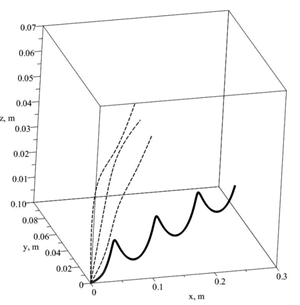
\includegraphics[width=0.5\linewidth]{Exp_BPR_3.png}
		\caption{Теоретическая (сплошная линия) и экспериментальные (штриховые линии) траектории движения безвинтового подводного робота $\bK=(2i_1\omega_{max}, 2i_2\omega_{max}, 0 )$} \label{traj3}
	\end{center}
\end{figure}

%\subsection{Выводы} при первых двух вариантах управляющих воздействий в рамках теоретической модели робот движется прямолинейно не изменяя своей ориентации. При проведении экспериментов такого движения добиться не удается.
Отметим, что при первых двух вариантах управляющих воздействий в рамках теоретической модели робот движется прямолинейно не изменяя своей ориентации. При проведении экспериментов такого движения добиться не удается. Так же перемещение безвинтового подводного робота на практике в два раза меньше, чем в теории. Более того в эксперименте при управляющем воздействии $\bK=\begin{pmatrix} 0,  2i_2\omega_{max}, 0 \end{pmatrix}$ движение робота происходит вдоль оси симметрии винтового тела (вдоль большей оси эллипсоида), а в теории робот движется перпендикулярно ей. 

\section{Выводы по экспериментам}

Анализируя отклонения и характер движения безвинтового подводного робота в экспериментах, можно сделать следующие выводы:

\begin{enumerate}
	\item	Управляемое движение безвинтового подводного робота на практике продолжается до тех пор, пока обеспечивается ускоренное вращение роторов. Чем больше ускорение роторов, тем быстрее движется робот. Однако, технически, максимальная угловая скорость вращения роторов ограничена, и после ее достижения робот продолжает движение по инерции.
	\item Разгон маховиков до максимальной скорости занимает определенное время (разгон большего маховика --- $t=0.9$ секунды, разгон малого маховика --- $t=0.7$ секунды), что не учитывается в теоретической модели и вносит свой вклад в траекторию движения безвинтового подводного робота.
	\item	Движение безвинтового подводного робота сопровождается образованием вихревых структур, что подтверждается данными, полученными с использованием системы визуализации потоков (PIV --- Particle Image Velocimetry). На рисунке \ref{piv} изображены линии вихрей в вертикальной плоскости при движении эллипсоида в жидкости. Обеспечить безвихревое движение, как этого требует теория (см. \cite{Vetchanin_Mamaev_Tenenev_RCD_2013, Ramodanov_Tenenev_Treschev_RCD_2012}) с помощью роторов крайне затруднительно. Необходимо использовать модифицированные уравнения движения, учитывающие циркуляцию вокруг тела \cite{Kilin_Vetchanin_DAN_2016}.
	
	\begin{figure}[h!]
		\begin{center}
			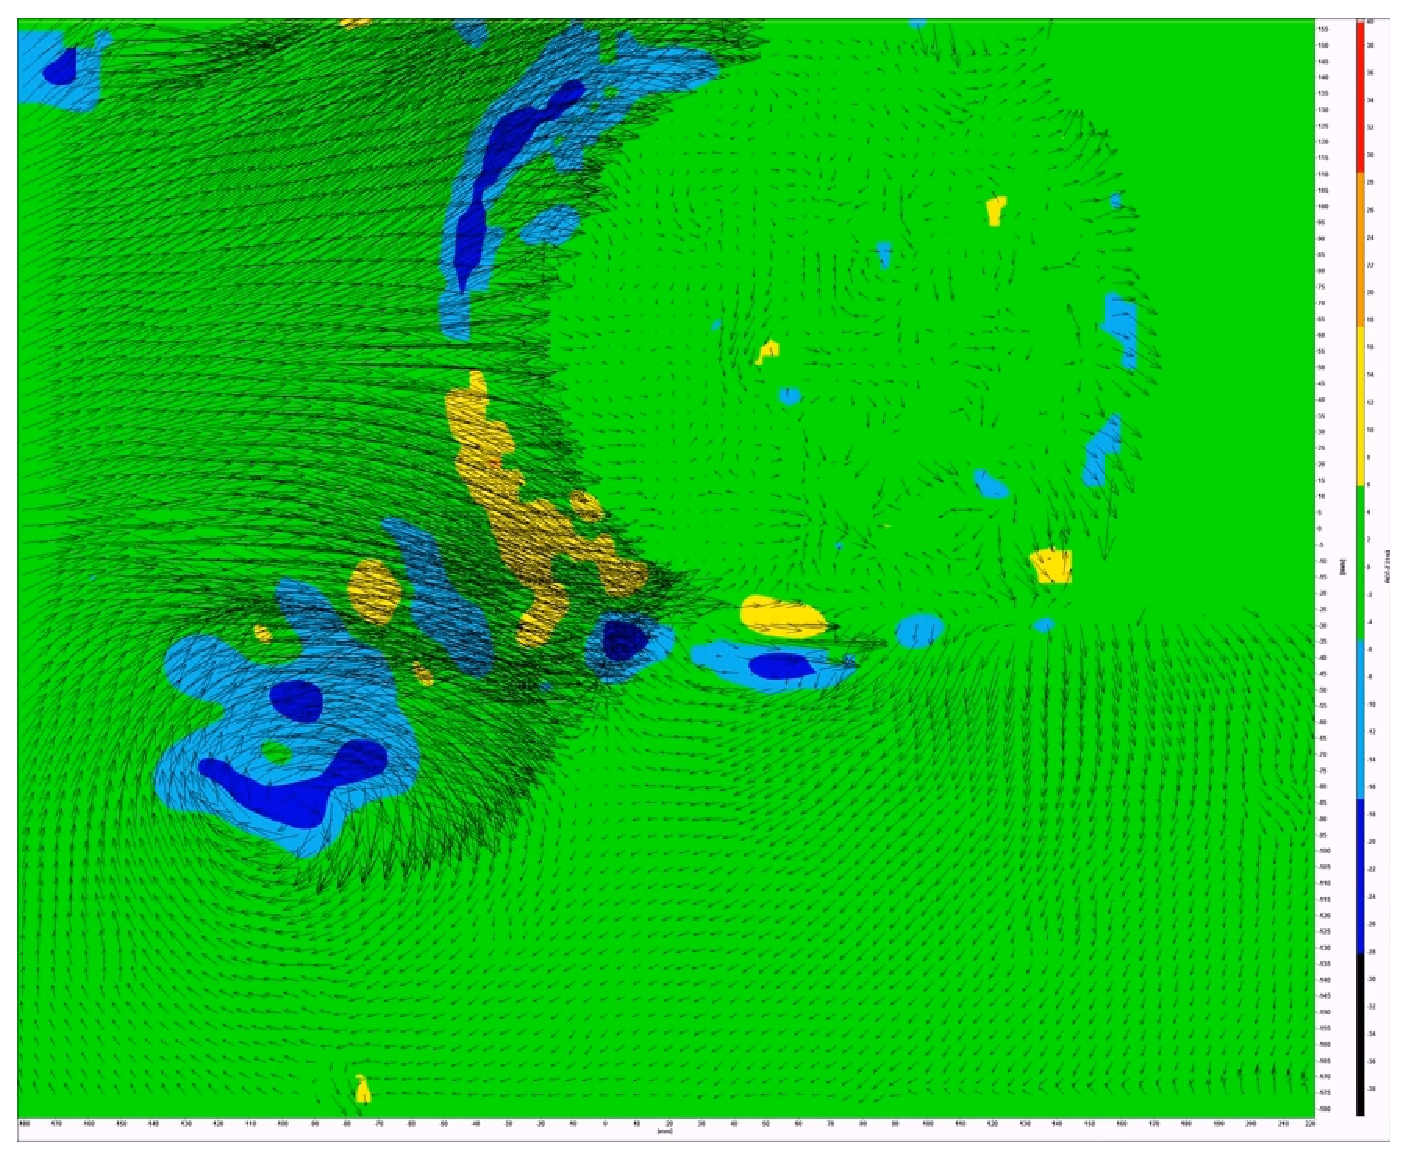
\includegraphics[width=0.4\linewidth]{piv.eps}
			\caption{Линии вихрей при движении эллипса в жидкости} \label{piv}
		\end{center}
	\end{figure}
	
	\item В теоретической модели используется идеализированная модель вязкости, что так же вносит несоответствия теоретической и реальной траектории движения.
	\item Подобную схему и алгоритмы управления в качестве практического применения можно использовать для реализации различных маневров (например, разворот на месте) в управлении подводными роботами.
	\item Модель качественно описывает движение, но на количественное согласование влияет точность определения большого количества параметров. Движение возможно, однако, его эффективность не высока.

\end{enumerate}

Учитывая полученные результаты, принято решение разработать вторую модель водного робота с внутренним ротором используя следующие тезисы:

\begin{enumerate}
	\item Использовать модель движения, учитывающую вязкое сопротивление жидкости, так как коэффициенты вязкого сопротивления существенно влияют на траекторию движения. Используя такую модель, для упрощения расчетом рассмотрим плоско-параллельное движение на поверхности жидкости.
	
	\item Использовать ассиметричную форму оболочки робота. При движении с образованием вихревых структур необходимо выбрать такую форму оболочки робота для которой образование вихрей не будет препятствовать движению. Такой формой может быть оболочка с острой кромкой, например, в виде профиля крыла Жуковского.
	
	\item Использовать периодическое управление. Движение робота происходит при ускоренном вращении роторов, а чтобы обеспечивать такое вращение необходимо периодически изменять направление вращения ротора. 
	
\end{enumerate}


	
	
\clearpage